\documentclass{beamer}
\usepackage[utf8]{inputenc}
\usepackage{graphicx}
\usepackage{color}
%\usetheme{Hannover}
\newcommand{\hilight}[1]{\textbf{\textcolor{structure.fg!85}{#1}}}
\setbeamertemplate{footline}[frame number]

\usepackage{hyperref}
\hypersetup{
    colorlinks=true,
    linkcolor=blue,
    filecolor=magenta,      
    urlcolor=cyan,
}

\author[Sowmya Vajjala]{Sowmya Vajjala}

\title[SfSNLP]{NLP without Annotated Dataset}
\subtitle{Course Review}


\date{29 January 2021}

\institute{Seminar f\"ur Sprachwissenschaft, University of T\"ubingen, Germany}
%%%%%%%%%%%%%%%%%%%%%%%%%%%

\begin{document}

\begin{frame}\titlepage
\end{frame}

\begin{frame}
\frametitle{Topics we covered}
\begin{enumerate}
\item NLP Overview
\item NLP system development pipeline
\item Corpus collection, extraction, exploration 
\item Automatically labeling data
\item Snorkel: Spam Classification without annotated data, Data augmentation with annotated data
\item Text Embeddings and Transfer Learning: An overview
\item Other shorter topics: NLP for Endangered Languages, NLP for Language Learning
\item Group Discussions on various topics. 
\end{enumerate}
\end{frame}

%a slide for each topic?
\begin{frame}{NLP Overview}
    \begin{itemize}
        \item Different faces of NLP: Research, Industry, Other disciplines
        \item Various day to day applications
        \item Challenges with NLP
        \item Some common tasks and
        \item Degrees of language processing
    \end{itemize}
\end{frame}

\begin{frame}{NLP Pipeline}
    \begin{itemize}
        \item How does one build NLP based software?
        \item How do we represent text for NLP?
        \item A real world case study
        \item A code walk through of the pipeline
    \end{itemize}
\end{frame}

%a slide for each topic?
\begin{frame}{Corpus collection, extraction, exploration}
    \begin{itemize}
        \item How can we get data for NLP?
        \item How do we extract text from various file formats?
        \item What is inside our corpus?
        \item What are some issues to consider while developing/using a corpus?
    \end{itemize}
\end{frame}

\begin{frame}{Automatic Data Creation}
    \begin{itemize}
        \item Different ways of labeling data
        \item Weak supervision
        \item Data augmentation
        \item Other topics:
        \begin{itemize}
            \item Text anonymization
            \item Text classification
        \end{itemize}
    \end{itemize}
\end{frame}

\begin{frame}{Snorkel}
    \begin{itemize}
        \item Generating training data for spam classification
        \item Using text augmentation for improving spam classification
    \end{itemize}
\end{frame}

\begin{frame}{Text Embeddings and Transfer Learning}
    \begin{itemize}
        \item Bag of words to BERT
        \item What happens during fine-tuning?
    \end{itemize}
\end{frame}

\begin{frame}{Other Topics}
    \begin{itemize}
        \item NLP for Endangered Languages
        \item NLP for Language Learning
        \item NLP careers
        \item Lot of interesting discussion papers
    \end{itemize}
\end{frame}

\begin{frame}{Graded Part}
\begin{itemize}
    \item Assignments
    \item Group discussion (DONE!)
    \item Term paper
    \item Classroom participation (DONE!?)
\end{itemize}    
\end{frame}

\begin{frame}{Some Ideas for Termpaper}
I am taking text classification as an example a I covered it in class 
    \begin{itemize}
        \item Compare different data augmentation methods for a simple text classification task
        \item Explore different *BERT models for a simple task
        \item Generating a labeled dataset for some new classification/IE task with Snorkel
        \item Surveying existing resources and software for a new language, and listing a few directions on how to extend them
        \item Exploring already existing datasets for its coverage, identifying potential issues with using it etc (e.g., following datasheets paper)
        \item Evaluating an existing tool (e.g., Spacy NER) in terms of how it does for various categories of text, using standard evaluation sets. 
    \end{itemize}
    .... .... 
\end{frame}

\begin{frame}
\frametitle{Initial ideas: Course Objectives}
\begin{itemize}
\item Provide an overview of NLP system development pipeline
\item Discuss some common approaches for collecting, cleaning and exploring text data
\item Introduce some methods to develop labeled data for NLP 
\end{itemize}
\end{frame}

\begin{frame}
\frametitle{Initial ideas: Learning Outcomes}
Students should be able to: 
\begin{itemize}
\item Understand the end to end NLP system development pipeline
\item Compile and explore labeled/annotated corpora for NLP
\item Build some basic text classification and information extraction systems
\end{itemize}
... upon successful completion of the course..
\end{frame}

\begin{frame}
\frametitle{Initial ideas: What the course can't do}
\begin{itemize}
\item Don't expect to become an NLP expert with one compact course. 
\item Contents may not always meet your own expectations, but there is a term paper and a group discussion, which gives you opportunities to explore your specific interests related to this topic.
\item The course won't teach you programming. 
\end{itemize}
\end{frame}

\begin{frame}{Upcoming Deadlines}
    \begin{itemize}
        \item March 1st: Assignments, Term paper
        \item Today: Make a decision on whether or not you want to submit a term paper, and let me know! (thanks for those who already informed!)
        \item Soon: Start working on assignments and term paper!
    \end{itemize}
\end{frame}

\begin{frame}
\frametitle{How we learn and grow}
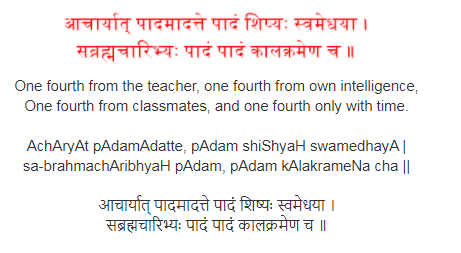
\includegraphics[width=\textwidth]{figures/acharyat.PNG}
\href{https://blog.practicalsanskrit.com/2009/12/how-we-learn-and-grow.html}{Source}
\end{frame}

\begin{frame}{Thank you!}

contact: sowmya.vajjala @ nrc-cnrc.gc.ca

Feel free to connect on social networks (Linkedin, twitter etc) if you want to (finding me is up to you)

\Large Wish you all good luck!!
\end{frame}

\end{document}